\chapter{Diseño de un Controlador de Velocidad}

Debido a las características de velocidad y precisión que ofrecen, los motores lineales pueden superar las especificaciones de métodos de movimiento lineal convencionales, como el uso de motores rotativos, engranajes, correas y poleas, cuando son utilizados en conjunto con sistemas de control de posición y/o velocidad. Un motor lineal, como sistema dinámico, es un sistema sujeto a ruido y perturbaciones
externas, como variaciones en la carga, por lo que existe una gran variedad de estrategias de control aplicables de acuerdo a su topología y a los requisitos del sistema controlado. Teniendo encuenta lo anterior, se analizaron las posibles estrategias de control para desarrollar el último objetivo del presente trabajo, que consiste en el diseño de un controlador de velocidad para el MLR obtenido junto con una simulación del mismo. Partiendo del control de campo orientado, se evaluaron dos estrategias aplicables a esta situación, y posteriormente se seleccionó una con la cual se diseñó el sistema de control y se verificó por medio de simulación, como se muestra a continuación.


\section{Evaluación de estrategias de control}
Existen diversas estrategias de complejidad variable que han sido aplicadas en el control de motores lineales y que han producido resultados satisfactorios, como el control robusto, óptimo y por medio de redes neuronales \cite{chen2007,liu2007,lopez2013}. Las estrategias seleccionadas para su evalación se escogieron debido a la efectividad que han mostrado en trabajos previos, y a la experiencia con que se contaba con las mismas. Estas se describen a continuación.

\subsection{Control de campo orientado}
El control de campo orientado (CCO) (también conocido como \textit{field oriented control} o FOC), es una alternativa al control de velocidad en motores síncronos por medio de la operación a \textit{volts por hertz constantes}, donde la velocidad del motor varía de acuerdo a la frecuencia, y el voltaje se varía p de mantener una razón voltaje-frecuencia constante, dado que en este modo  los cambios arbitrarios en la frecuencia no pueden ser seguidos por el motor con facilidad \cite{fitzgerald2003}. El CCO utiliza la descomposición de las cantidades en el motor en sus componentes en directo y en cuadratura (véase la sección B.2 del apéndice B). Esta descomposición es particularmente útil en motores de reluctancia variable como el MLR diseñado, debido a que se simplifica la relación entre la inductancia y la posición del motor, produciendo un modelo matemático que, como se verá más adelante, puede utilizarse fácilmente para el diseño de sistemas de control con diferentes estrategias \cite{boldea2013}.

La ecuación fundamental del MLR indica que el empuje desarrollado está dado por
\begin{equation}
F_x = \frac{3\pi}{2\tau}(L_d - L_q)i_d i_q
\end{equation}
Desde el punto de vista del control del empuje en el MLR, puede decirse que existe un grado de libertad en el mismo, dado por el producto $i_d i_q$. De esta forma, se puede establecer un valor de referencia para la corriente en el eje directo de acuerdo a su valor nominal (que para el MLR diseñado es de 2 A), mientras que la corriente de referencia en el eje en cuadratura puede ser determinada por un lazo de realimentación de velocidad, como se muestra en la Fig. \ref{fig:constantid}. Esta técnica de control se conoce como \textbf{control vectorial con $i_d$ constante} \cite{betz1993}, y produce sistemas de lazo cerrado con una respuesta de torque rápida \cite{jeanpaul2011}.

\begin{figure}[t]
\centering
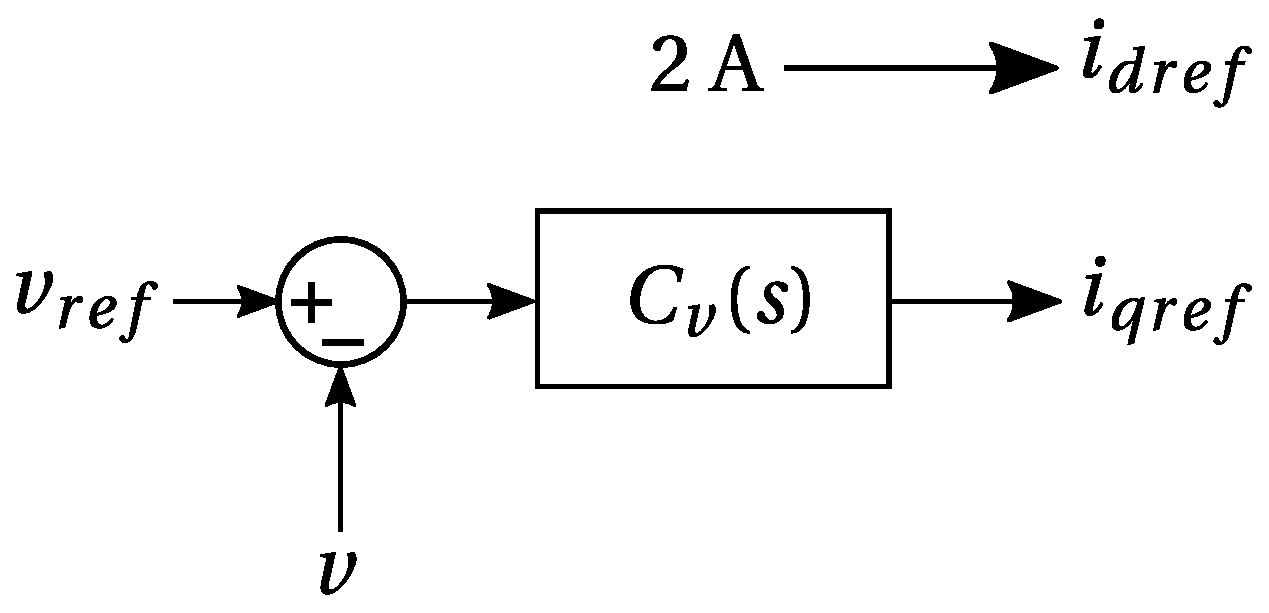
\includegraphics[scale=0.285]{../img/Diseno_de_un_controlador_de_velocidad/constantid.eps}
\caption{Control vectorial con $i_d$ constante, donde $v$ es la velocidad de desplazamiento medida del MLR.}
\label{fig:constantid}
\end{figure}

Lo anterior indica que es necesario establecer lazos de control en dos niveles: un lazo de control de corriente para controlar las corrientes en los ejes directo y en cuadratura, y un lazo externo de control de velocidad. Estos lazos de realimentación se pueden construir utilizando diferentes estrategias de control, de las cuales depende el método de diseño y operación de los mismos. En este trabajo se examinaron dos posibles estrategias de control: el control clásico y el control difuso, como se expone a continuación.

\subsection{Control clásico}
El control clásico parte del modelamiendo de sistemas dinámicos por medio de ecuaciones diferenciales lineales, que mediante la transformada de Laplace, brindan información sobre su comportamiento transiente y en estado estacionario, y que simplifican el diseño de controladores para los mismos, que actúan sobre el error en el sistema de control de forma proporcional, integral y derivativa, o una combinación de estos, en lo que se conoce como control proporcional (P), proporcional-integral (PID) o proporcional-integral-derivativo (PID), entre otros \cite{ogata2010}. Existen varias técnicas de diseño en el control clásico, como el método de Ziegler-Nichols \cite{ogata2010}, el método del lugar geométrico de las raíces (LGR) y el diseño en el dominio de la frecuencia \cite{chen1993}.

\begin{figure}[t]
    \centering
    \begin{subfigure}[b]{0.49\textwidth}
    \centering
        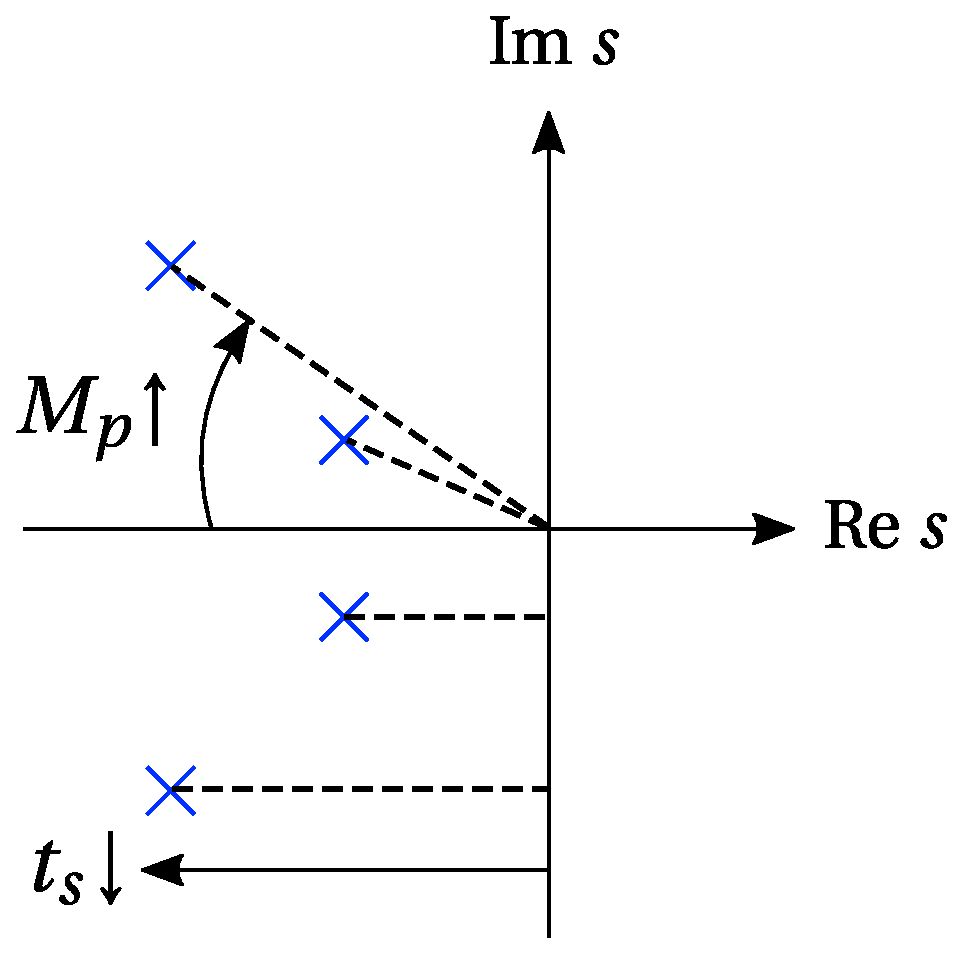
\includegraphics[scale=0.25]{../img/Diseno_de_un_controlador_de_velocidad/lgr.eps}
        \caption{Relación entre la posición de los polos y las características del sistema}
        \label{fig:lgr}
    \end{subfigure}
    ~ %add desired spacing between images, e. g. ~, \quad, \qquad, \hfill etc. 
      %(or a blank line to force the subfigure onto a new line)
    \begin{subfigure}[b]{0.49\textwidth}
    \centering
        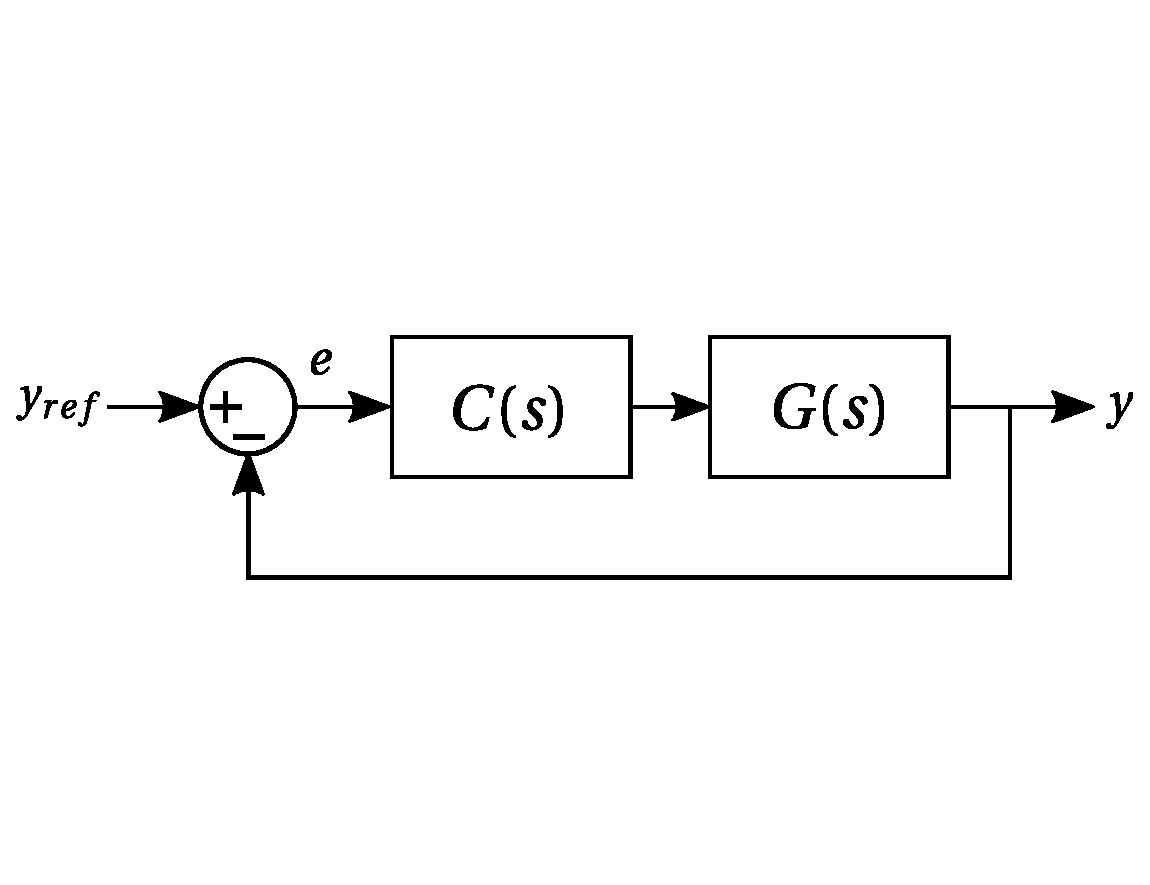
\includegraphics[scale=0.3]{../img/Diseno_de_un_controlador_de_velocidad/feedback.eps}
        \caption{Lazo de realimentación negativa}
        \label{fig:feedback}
    \end{subfigure}
    \caption{LGR y configuración del sistema con el controlador.}\label{fig:lgrfeedback}
\end{figure}

El método del LGR puede llevarse a cabo manualmente a partir del análisis de la posición de los polos y ceros en el plano $s$ del sistema a controlar. Estas posiciones tienen un efecto en la respuesta de lazo cerrado del sistema, como se muestra en la Fig. \ref{fig:lgr}. Por medio de la realimentación negativa y el uso de un controlador $C(s)$ en el mismo, como se muestra en la Fig. \ref{fig:feedback}, es posible obtener un nuevo sistema con polos cuyas posiciones permiten obtener un sistema de lazo cerrado que cumpla ciertos requisitos. La estructura de $C(s)$ puede ser simplemente una ganancia (un controlador tipo P), o controladores más elaborados, como PI, PID o compensadores.

Debido a que la transformación de Park permite obtener ecuaciones diferenciales lineales para los ejes directo y en cuadratura (como se muestra en el apéndice B), el control clásico es ampliamente aplicado en el CCO hasta años recientes, incluyendo aplicaciones de control de motores lineales, para los cuales el control de tipo PI es generalmente utilizado \cite{ramana2015,cheema2013,motlagh2012,gu2003}, en los que se implementan los lazos de corriente y velocidad mencionados anteriormente por medio de este tipo de controlador, para seguir un valor de referencia de velocidad. En aplicaciones de movimiento lineal, es posible incluso evitar el uso de un sensor de posición, al realizar una estimación de la posición del motor a partir de las corrientes y voltajes medidas (utilizadas en los lazos de realimentación) \cite{cheema2013}.

\subsection{Control difuso}

La lógica difusa \cite{zadeh1965} puede tomarse como una generalización de la lógica clásica, en la cual la pertenencia de un conjunto puede tomar uno de dos valores, dependiendo de si el elemento pertenece o no al conjunto \cite{wang1997}. En la lógica difusa, la función de pertenencia a un conjunto difuso puede tomar valores en el intervalo $[0, 1]$, como se muestra en la figura \ref{fig:fuzzymf}, donde se representan tres conjuntos difusos para diferentes valores de temperatura.

\begin{figure}[b]
\centering
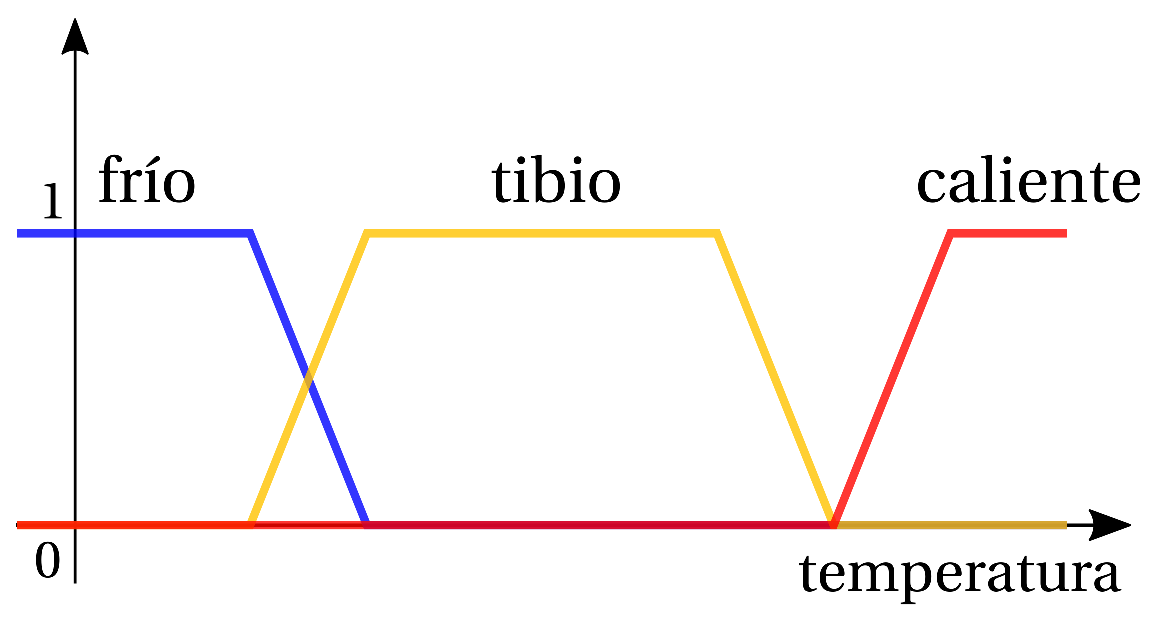
\includegraphics[scale=0.3]{../img/Diseno_de_un_controlador_de_velocidad/fuzzymf.eps}
\caption{Funciones de pertenencia para tres conjuntos difusos}
\label{fig:fuzzymf}
\end{figure}

La lógica y las operaciones matemáticas difusas permiten establecer una base para formalizar el conocimiento humano en forma de reglas \textbf{si-entonces} (\textit{if-then}). Mientras que con el control clásico el diseño inicia con un modelo matemático del proceso a controlar para el cual el controlador es diseñado, el control difuso inicia con una heurística y el conocimiento de un humano experto en forma de reglas si-entonces \cite{wang1997}, de forma que el controlador sintetice estas reglas. El conocimiento del experto humano puede provenir, por ejemplo, de un operador que haya actuado previamente como un elemento en el sistema de control, o un ingeniero que ha modelado matemáticamente el proceso y ha realizado un análisis sobre su comportamiento \cite{passino1998}.

Los controladores difusos pueden ser de dos tipos: no adaptativos o adaptativos. Mientras que en el control difuso no adaptativo los parámetros del controlador se fijan al inicio de la operación, el control aptativo está sujeto a cambios en tiempo real. El primer tipo es más sencillo pero requiere de más reglas, mientras que el segundo es más complejo pero requiere menos conocimiento de la planta y puede presentar un mejor desempeño \cite{wang1997}. En el caso de los motores lineales, se ha propuesto el uso de controladores difusos, que presentan una alternativa a estrategias de control donde se requiere un modelo matemático de la planta, utilizando técnicas como control de modo deslizante difuso (\textit{fuzzy sliding mode control}) \cite{zhao2007} y adaptativo \cite{lin2008}, para aplicaciones de control de posición \cite{chen2011}\cite{chen2005} y de velocidad \cite{linsen2007}.

\subsection{Selección de la estrategia de control}

Tanto para el control clásico como el difuso, los trabajos revisados indican que el CCO es el método a seguir al trabajar con motores de corriente alterna, debido a que el control de volts por hertz constante se utiliza principalmente para el arranque y apagado de motores, mientras que para aplicaciones de velocidad variable se prefiere el uso del CCO.

El control difuso ofrece la ventaja de permitir el diseño de un sistema de control sin un conocimiento específico de la función de transferencia del sistema, al incluir la experiencia de un operario o introducir el aprendizaje del modelo dentro del sistema de control. Sin embargo, en el presente caso, ya se cuenta con un modelo matemático del MLR a controlar, lo cual incluye el valor de las inductancias en los ejes directo y en cuadratura, la resistencia del primario y la masa del motor, y además, no se cuenta con una experiencia sobre la operación del motor que sirva como criterio para diseñar un sistema difuso útil en un sistema de control. Por estas razones se decidió aplicar la teoría del control clásico para el diseño de un controlador de velocidad del MLR, teniendo en cuenta además que es una herramienta que aún es relevante y confiable en el control de máquinas eléctricas, como indican los trabajos encontrados en el área.

\section{Metodología}

El primer paso para iniciar con el diseño de un controlador consiste en la obtención de un modelo matemático para el sistema. Como se muestra en el apéndice B, la transformación de Park permite obtener las ecuaciones diferenciales para el voltaje en los ejes directo $v_d$ y en cuadratura $v_d$:
\begin{align*}
v_d &= R_s i_d + L_d\frac{di_d}{dt} - v_{me}L_q i_q\\
v_q &= R_s i_q + L_q\frac{di_q}{dt} + v_{me}L_d i_d
\end{align*}
De estas ecuaciones se observa que existen dos términos que acoplan las dos ecuaciones de cada uno de los ejes: $v_{me}L_q i_q$ y $v_{me}L_d i_d$. En las ecuaciones diferenciales, estos términos pueden considerarse como perturbaciones que ocurren en cada eje y que los lazos de control tienen que corregir \cite{jeanpaul2011}. Entonces las ecuaciones desacopladas en cada eje pueden escribirse como sigue:
\begin{align}
v_d &= R_s i_d + L_d\frac{di_d}{dt}
\label{daxiseq}\\
v_q &= R_s i_q + L_q\frac{di_q}{dt}
\label{qaxiseq}
\end{align}

La ecuación fundamental del MLR relaciona el empuje con las corrientes en los ejes directo y en cuadratura:
\begin{equation}
F_x = \frac{3\pi}{2\tau}(L_d - L_q)i_d i_q
\label{thrusteq}
\end{equation}

Por último, el movimiento del motor está gobernado por la segunda ecuación de Newton, de acuerdo al siguiente diagrama:
\begin{figure}[hbtp]
\centering
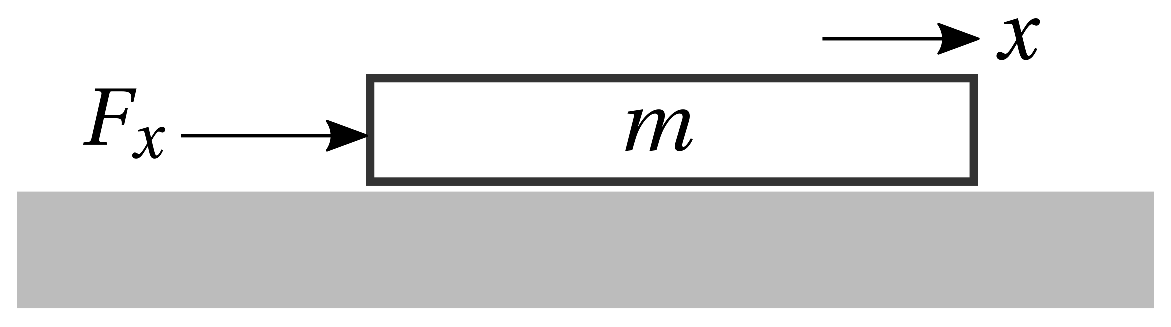
\includegraphics[scale=0.25]{../img/Diseno_de_un_controlador_de_velocidad/displacement.eps}
\end{figure}

Si se desprecia la fricción viscosa, se obtiene la siguiente relación:
\begin{equation}
F_x = m\frac{d^2x}{dt^2}
\label{displacementeq}
\end{equation}

Las ecuaciones \ref{daxiseq} a \ref{displacementeq} forman un modelo matemático del sistema a partir del cual se procede a diseñar un sistema de control utilizando la teoría de control clásico. Como se observa en estas ecuaciones, existen una serie de parámetros fijos (mecánicos y eléctricos) asociados con el sistema. Estos valores se obtuvieron durante el proceso de diseño y optimización del motor y se listan en la Tabla \ref{table:mlrparams}.

\begin{table}[t]
\centering
\caption{Parámetros del modelo matemático del MLR.}
\label{table:mlrparams}
\begin{tabular}{c c c}\hline
Símbolo & Descripción & Valor\\
\hline\hline
$L_d$ & Inductancia del eje directo & 0.614 H\\
$L_q$ & Inductancia del eje en cuadratura & 0.128 H\\
$R_s$ & Resistencia del primario & 7.62 $\Omega$\\
$\tau$ & Paso polar & 12 cm\\
$m$ & Masa del primario y carga & 6.6 kg
\end{tabular}
\end{table}

Aplicando la transformada de Laplace, se obtienen las funciones de transferencia de voltaje a corriente en los ejes directo $G_d(s)$ y en cuadratura $G_q(s)$, así como la función de transferencia de empuje a desplazamiento $G_{fx}(s)$. Por un lado, se obtuvieron funciones de transferencia de primer orden para $G_d(s)$,
\begin{equation*}
\frac{I_d(s)}{V_d(s)} = G_d(s) = \frac{1/R_s}{1+\frac{L_d}{R_s}s} =
\frac{0.1312}{1+0.0806s}
\end{equation*}
y $G_q(s)$:
\begin{equation*}
\frac{I_q(s)}{V_q(s)} = G_q(s) = \frac{1/R_s}{1+\frac{L_q}{R_s}s} =
\frac{0.1312}{1+0.0168s}
\end{equation*}

Por otro lado, para la función de transferencia $G_{fx}(s)$ se obtuvo una función de segundo orden con dos polos repetidos en el origen. Si se incluyen los factores constantes de la ecuación \ref{thrusteq} en esta función de transferencia, se tiene que
\begin{equation}
\frac{X(s)}{F(s)} = G_{fx}(s) = \frac{K}{ms^2}
\end{equation}
donde $K = \frac{3\pi}{2\tau}(L_d - L_q)$.

Una vez definidas las funciones de transferencia del sistema, se examinó su respuesta en lazo abierto, como se muestra en la Fig. \ref{fig:openloop}. En esta se observa que el tiempo de establecimiento en el eje en cuadratura (de 65 ms) es más bajo que el del eje directo (310 ms), debido a la baja inductancia que se presenta en el eje en cuadratura en los MLR, en comparación con la inductancia del eje directo. Además, se observa que existe un alto error de posición (dada una entrada unitaria).

Con el fin de que la influencia de las corrientes $i_d$ e $i_q$ tenga el mismo comportamiento en el tiempo sobre el empuje producido por el motor, se decidió que los lazos de control debían producir una constante de tiempo igual en ambos ejes, de 100 ms (un valor arbitrario entre los valores de tiempo de establecimiento obtenidos en lazo abierto), error de posición de cero, y un sobrepaso máximo de 2\%. Los controladores para cada eje se diseñaron por medio del método del lugar geométrico de las raíces.

\begin{figure}[t]
\centering
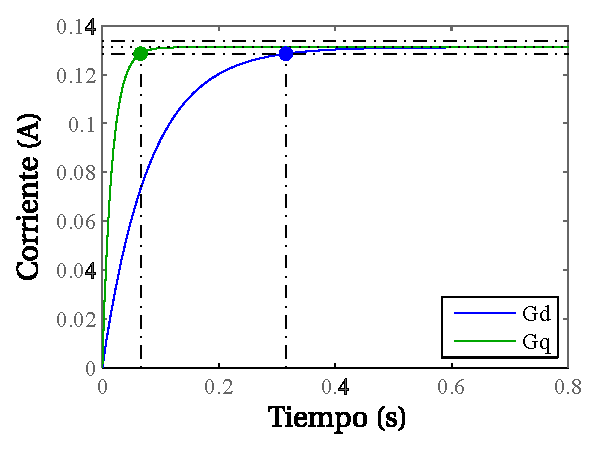
\includegraphics[scale=0.8]{../img/Diseno_de_un_controlador_de_velocidad/openloop.eps}
\caption{Respuesta en lazo abierto de $G_d(s)$ y $G_q(s)$, indicando los tiempos de establecimiento.}
\label{fig:openloop}
\end{figure}

Para el lazo externo de control de velocidad, se asumió que que los tiempo de respuesta de las variables eléctricas eran mucho menores a las constantes de los tiempos de las variables mecánicas \cite{jeanpaul2011}, de forma que las corrientes siguen instantáneamente la señal de control producida por el controlador de corriente. Para este controlador los requisitos definidos fueron error de posición cero, sobrepaso máximo de cero y un tiempo de establecimiento de 2 segundos, el cual igualmente fue diseñado por medio del método del lugar geométrico de las raíces.

Una vez se obtuvieron los controladores, se procedió a realizar una simulación del sistema completo, incluyendo los lazos de realimentación y de corriente junto con la carga del motor, por medio del software Simulink.

\section{Resultados}
El proceso de diseño de los controladores por medio del lugar geométrico de las raíces se realizó manualmente, de forma que fue necesario sintonizar la respuesta e intentar con controladores de tipo PI y PID hasta obtener la respuesta deseada. Finalmente, los controladores de corriente para los ejes directo $C_d(s)$ y en cuadratura $C_q(s)$ obtenidos fueron de tipo PID, cuya función de transferencia es la siguiente:
\begin{align*}
C_d(s) &= \frac{0.05(15.568+s)(358.432+s)}{s}\\
C_q(s) &= \frac{0.0175(124.531+s)(132.612+s)}{s}
\end{align*}

\begin{figure}[t]
\centering
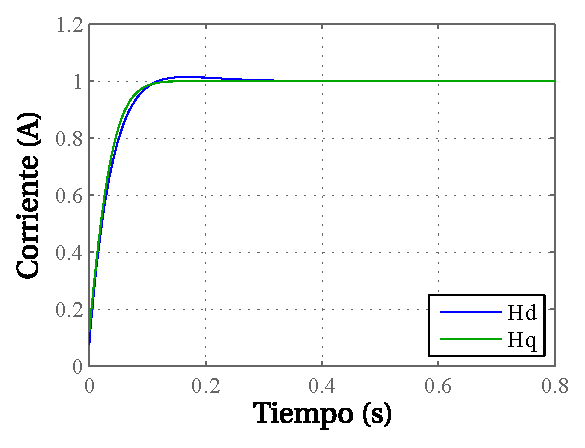
\includegraphics[scale=0.8]{../img/Diseno_de_un_controlador_de_velocidad/closedloopcurrent.eps}
\caption{Respuesta en lazo cerrado de los lazos de corriente.}
\label{fig:closedloopcurrent}
\end{figure}

Utilizando estos controladores se obtuvo un sobrepaso máximo de 1.4\%, un tiempo de establecimiento de 100 ms y cero error de posición.

Con respecto al lazo de control de velocidad, fue suficiente diseñar un controlador proporcional, debido a los polos repetidos en el origen de la función de transferencia $G_{fx}(s)$. El método del lugar geométrico de las raíces permitió obtener el valor de la constante, de lo que se obtuvo
\begin{equation}
G_v(s) = 13.2
\end{equation}
La respuesta obtenida, mostrada en la Fig. \ref{fig:closedloopspeed}, mostró un tiempo de establecimiento de 2 segundos, cero sobrepaso y cero error de posición, como se había especificado.

\begin{figure}[hbtp]
\centering
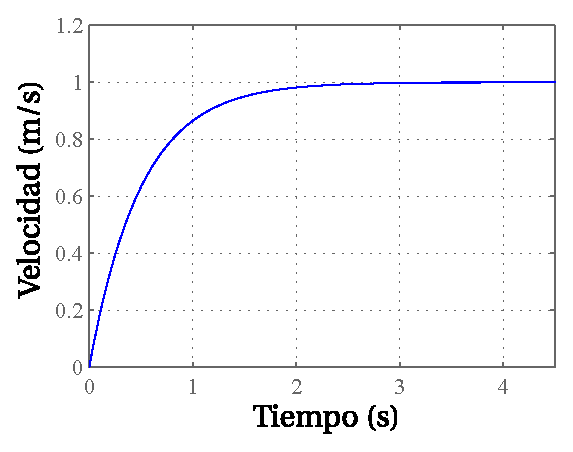
\includegraphics[scale=0.8]{../img/Diseno_de_un_controlador_de_velocidad/closedloopspeed.eps}
\caption{Respuesta en lazo cerrado del lazo de velocidad.}
\label{fig:closedloopspeed}
\end{figure}

Las respuestas anteriores se obtuvieron únicamente con las funciones de transferencia aisladas del resto del sistema. Con el fin de observar el comportamiento del sistema completo, incluyendo las funciones de transferencia en conjunto con la dinámica del motor (junto con los términos que acoplan las ecuaciones diferenciales de corriente en los ejes directo y en cuadratura), se realizó una simulación en Simulink, cuyo diagrama se muestra en la Fig. \ref{fig:closedloop}. A la salida de los controladores de corriente se añadieron bloques de saturación, para modelar el hecho de que estos valores deben estar limitados en una implementación del sistema de control, a un valor máximo de 2 A, el cual fue determinado durante la optimización del diseño.

Los resultados de la simulación se muestran en la Fig. \ref{fig:finalresponse}. Estos resultados se obtuvieron al especificar una entrada con diferentes valores de referencia que eran cambiados a lo largo del tiempo, durante un intervalo de 8 segundos. Estos resultados muestran como todo el sistema, teniendo en cuenta todos los efectos de acoplamiento y saturación de las corrientes, presenta un tiempo de establecimiento de 200 ms, el cual es menor al que se especificó durante el diseño del lazo de control de velocidad, que únicamente tenía en cuenta la dinámica de la masa del motor.

\begin{figure}[hbtp]
\centering
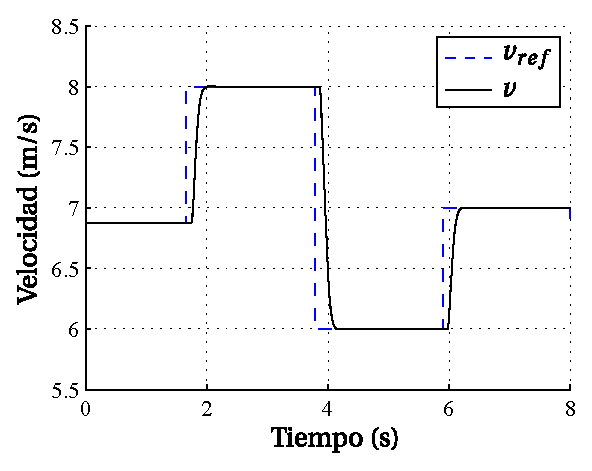
\includegraphics[scale=0.8]{../img/Diseno_de_un_controlador_de_velocidad/finalresponse.eps}
\caption{Resultados de la simulación del sistema completo en Simulink.}
\label{fig:finalresponse}
\end{figure}


\begin{figure}[!]
\centering
\rotatebox{90}{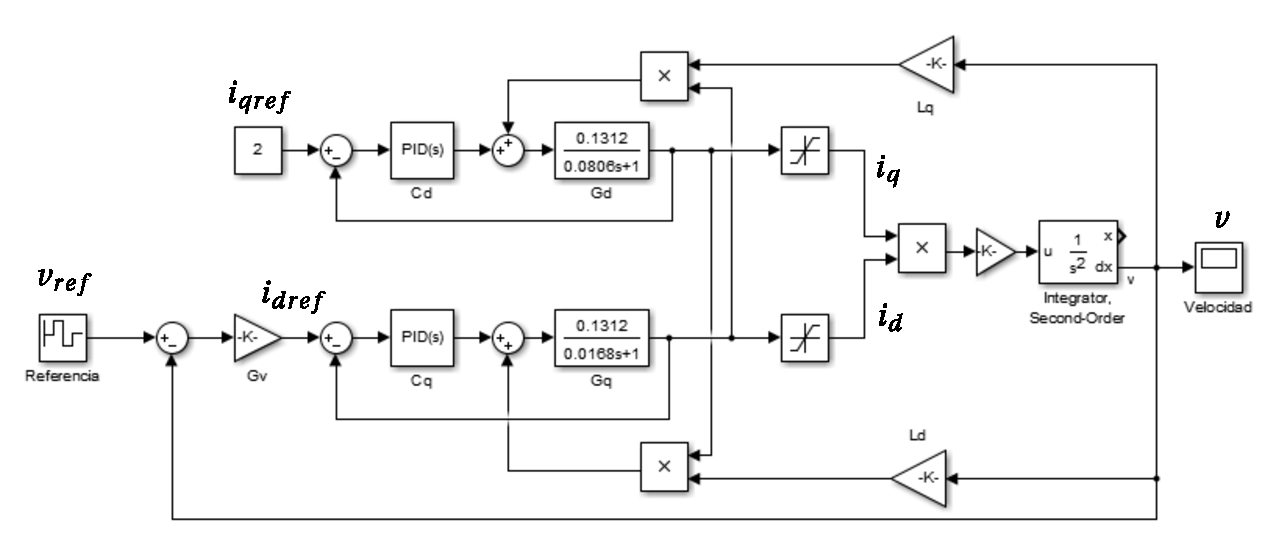
\includegraphics[width=1.40\linewidth]{../img/Diseno_de_un_controlador_de_velocidad/closedloop.eps}}
\caption{Geometría del MLR diseñado, mostrando el primario en su totalidad.}
\label{fig:closedloop}
\end{figure}

\section{Conclusiones}
Los resultados obtenidos con el CCO en conjunto con el control clásico indican que para aplicaciones de velocidad variable, estas técnicas son válidas y proveen métodos sencillos para el diseño de sistemas de control, una vez se cuenta con un modelo matemático del MLR. Esto se evidenció en el trabajo realizado, en el que las etapas de metamodelado y optimización brindaron los conocimientos necesarios para plantear un modelo matemático.

Aún cuando el diseño de cada controlador se hizo de manera aislada, asumiendo los efectos externos como perturbaciones, se observó a través de la simulación que el desempeño del sistema completo presentó variaciones, que mantuvieron el desempeño dentro de los requisitos establecidos.

Siendo incluso la teoría de control clásico una teoría antigua, la revisión del estado del arte y los resultados obtenidos muestran que existen aplicaciones relevantes en la actualidad en las cuales las estrategias de control desarrolladas a partir de esta funcionan satisfactoriamente, en comparación con estrategias que pueden resultar más complicadas en el contexto del problema.

\bibliographystyle{ieeetr}
\bibliography{../refs}